\documentclass{beamer}
\usepackage[utf8]{inputenc}
\usepackage{amsmath,amsfonts,amsthm,amstext,amssymb, xcolor, tikz, pgf}

% ----------------------------------------------------------
% Theme Setup

% Use Metropolis Theme
\usetheme[numbering=fraction]{metropolis}
\setbeamertemplate{blocks}[rounded][shadow=false]
\makeatletter
\setlength{\metropolis@titleseparator@linewidth}{1pt}
\makeatother



% Define Colors
\definecolor{chargerblue}{HTML}{002764}
\definecolor{chargerred}{HTML}{e02034}
\definecolor{bggray}{HTML}{d0d3d4}

% Set Colors
\setbeamercolor{title}{fg=chargerblue}
\setbeamercolor{background canvas}{bg=white}
\setbeamercolor{title separator}{fg=chargerred}
\setbeamercolor{structure}{fg=chargerblue}
\setbeamercolor{frametitle}{fg=white, bg=chargerblue}
\setbeamercolor*{normal text}{fg=chargerblue}
\setbeamercolor*{block body}{bg=bggray}
\setbeamercolor*{block title}{bg=chargerblue, fg=white}
% ----------------------------------------------------------

% ----------------------------------------------------------
% Custom Definitions, Commands, Environments, etc.

% Sets of numbers
\def\R{\mathbb{R}} % The reals
\def\N{\mathbb{N}} % The naturals
\def\Z{\mathbb{Z}} % The integers
\def\Q{\mathbb{Q}} % The rationals

% Blank space
\newcommand{\blank}[1]{\underline{\hspace{#1}}} % Blank space

% Fitted inclusion symbols
\newcommand{\fp}[1]{\left({#1}\right)} % Fitted parentheses around content
\newcommand{\fb}[1]{\left[{#1}\right]} % Fitted brackets
\newcommand{\set}[1]{\left\{{#1}\right\}} % Fitted braces (useful for sets)
\newcommand{\av}[1]{\left|{#1}\right|} % Fitted absolute value bars

% Coordinate Plane (Four-Quadrant)
\def\coordplane {
	\begin{tikzpicture}
		\draw[step=0.25cm,black,very thin,opacity=0.25] (-2.5cm, -2.5cm) grid (2.5cm, 2.5cm);
		\draw[<->,thick,black] (-2.5cm, 0) -- (2.5cm, 0) node[anchor=north west,pos=0.94,font=\scriptsize]{$x$};
		\draw[<->,thick,black] (0,-2.5cm) -- (0, 2.5cm) node[anchor=south east,font=\scriptsize,pos=0.94]{$y$};
	\end{tikzpicture}
}

% Coordinate Plane (One-Quadrant)
\def\onequad {
	\begin{tikzpicture}
		\draw[step=0.25cm, black, very thin, opacity=0.25] (0,0) grid (7.5cm,5cm);
		\draw[->, thick, black] (0,0) -- (7.5cm, 0) node[anchor=north west,font=\scriptsize,pos=0.94]{$x$};
		\draw[->, black, thick] (0,0) -- (0,5cm) node[anchor=south east,font=\scriptsize,pos=0.94]{$y$};
	\end{tikzpicture}
}
% ----------------------------------------------------------


% ----------------------------------------------------------
% Presentation Information 
\title[1.1 and 1.2]{Graphs of Equations; Linear Equations in One Variable}
\subtitle{Section 1.1 and 1.2}
\author{Jacob Ayers}
\institute{Lesson \#4}
\date{MAT 130}
% ----------------------------------------------------------

\begin{document}

% Slide 1 (Title Slide)
\begin{frame}
\titlepage
\end{frame}

% Slide 2 (Objectives)
\begin{frame}[t]{Objectives}
\begin{itemize}
	\item Graph equations by plotting points
	\item Find intercepts of equations
	\item Determine symmetry graphically and algebraically
	\item Solve linear equations in one variable
	\item Use linear equations to solve real-life problems
\end{itemize}
\end{frame}

\begin{frame}[t]{Determining Solution Points}
\begin{block}{Definition}
A point $(x,y)$ is a \textit{solution} to an equation if plugging $x$ and $y$ into the equation results in a true statement.
\end{block} \vspace{12pt}

\pause

Example: Determine whether $(-2, 26)$ is a solution to $y = 14 - 6x$.

\pause

$26 \stackrel{?}{=} 14 - 6(-2)$ \hspace{1in} YES \vspace{12pt}

\pause

Example: Determine whether $(3, 12)$ is a solution to $y = 2x^2 - 4x + 1$.

\pause

$12 \stackrel{?}{=} 2(3)^2 - 4(3) + 1$ \hspace{1in} NO
\end{frame}

\begin{frame}[t]{The Point-Plotting Method}
In this course, we'll see many methods of graphing specific types of function.

The point-plotting method of graphing will allow us to sketch the graph of any equation we want, provided we plot enough points.

\pause

\begin{block}{The Point-Plotting Method of Graphing}
\begin{enumerate}[1)]
\item Isolate one of the variables if possible
\item Construct a table of values with several solution points
\item Plot the points
\item Connect the points
\end{enumerate}
\end{block}
\end{frame}

\begin{frame}[t]{The Point-Plotting Method}
Sketch the graph of $-2x + y = 1$ using the point-plotting method.

\pause

1) Isolate a variable: $y = 2x + 1$

\pause

2) Construct a table of values:
\begin{tabular}{|c|c|c|}
\hline 
$x$ & $y = 2x + 1$ & $(x,y)$ \\ 
\hline 
-3 & -5 & $(-3, 5)$ \\ 
\hline 
-2 & -3 & $(-2, -3)$ \\ 
\hline 
-1 & -1 & $(-1,-1)$ \\ 
\hline 
0 & 1 & $(0,1)$ \\ 
\hline 
1 & 3 & $(1,3)$ \\ 
\hline 
2 & 5 & $(2,5)$ \\ 
\hline 
3 & 7 & $(3,7)$ \\ 
\hline 
\end{tabular} 
\end{frame}

\begin{frame}[t]{The Point-Plotting Method}
Sketch the graph of $-2x + y = 1$ using the point-plotting method.

3) Plot and connect the points

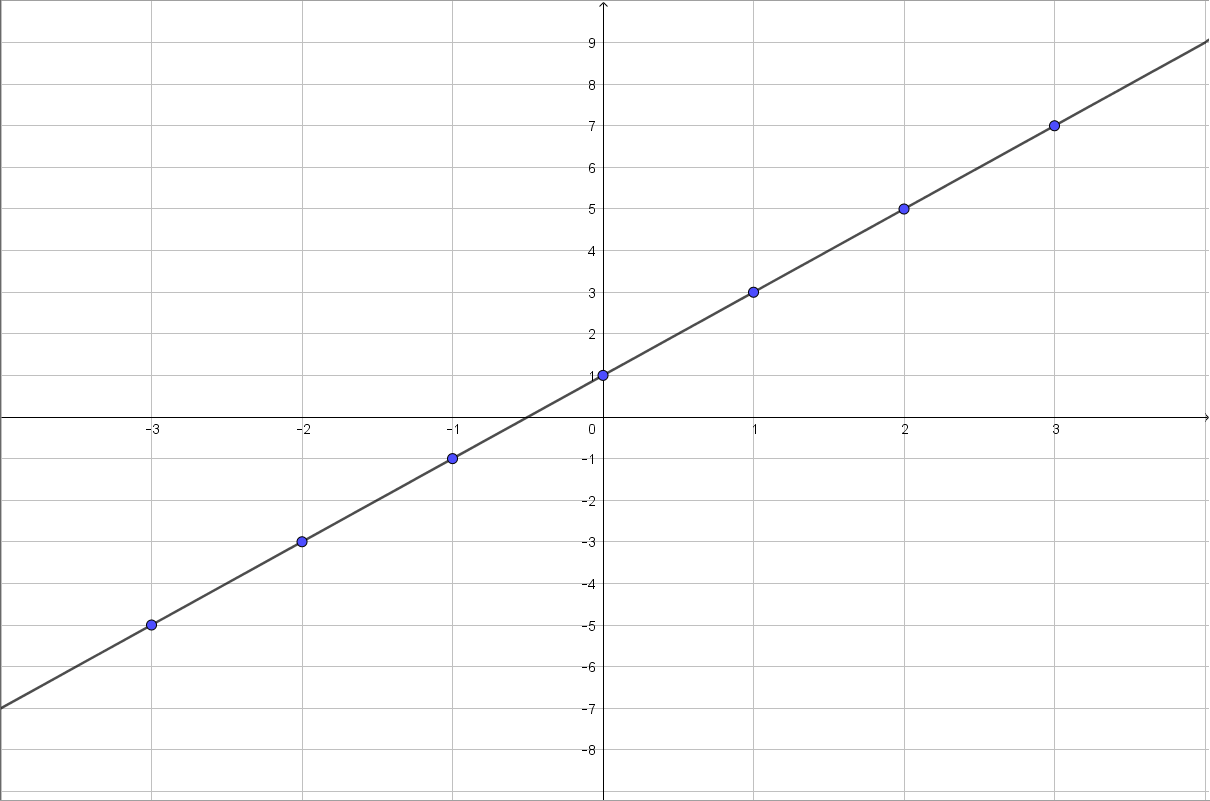
\includegraphics[width=3in]{GraphLine1.png}
\end{frame}

\begin{frame}[t]{Intercepts}
\begin{block}{Definition}
An \textit{intercept} of an equation is a solution point that is on the $x$-axis ($x$-intercept) or the $y$-axis ($y$-intercept).
\end{block}

\pause

To find intercepts graphically, just look for where the graph crosses each axis.

\pause

To find intercepts algebraically: \vspace{-6pt} \begin{itemize}
\item $x$-intercept: set $y = 0$ and solve for $x$
\item $y$-intercept: set $x = 0$ and solve for $y$
\end{itemize}
\end{frame}

\begin{frame}[t]{Intercepts}
Identify the intercepts of the graph below, which represents the equation $y = -x^2 - 5x$.

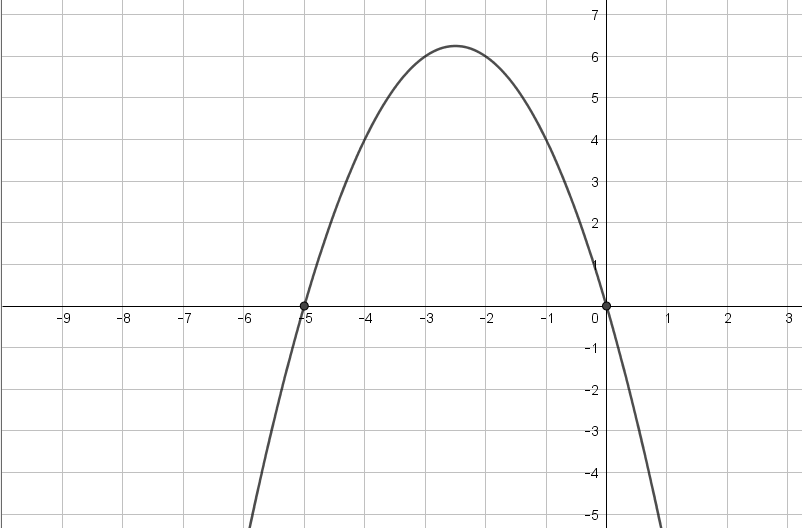
\includegraphics[width=2in]{GraphParabola1.png}

\pause

$x$-intercepts: $(-5,0)$, $(0,0)$ \\
$y$-intercept: $(0,0)$
\end{frame}

\begin{frame}[t]{Intercepts}
Find the intercepts of the equation $4x + 5y = 40$

\pause

$4x + 5(0) = 40 \Rightarrow 4x = 40 \Rightarrow x = 10$; the $x$-intercept is $(10,0)$

\pause

$4(0) + 5y = 40 \Rightarrow 5y = 40 \Rightarrow y = 8$; the $y$-intercept is $(0,8)$

\pause

Graph:

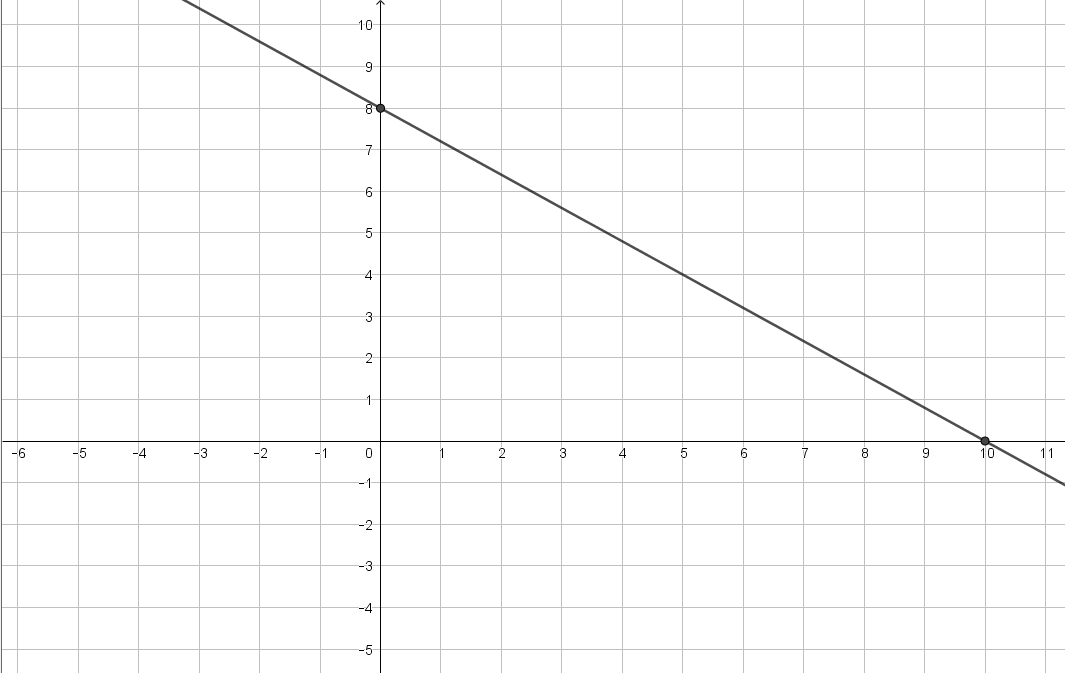
\includegraphics[width=2.5in]{GraphLine2.png}
\end{frame}

\begin{frame}[t]{Symmetry}
\begin{block}{Graphical Tests of Symmetry}
\begin{enumerate}[1)]
\item About the $x$-axis: whenever $(x,y)$ is on the graph, $(x,-y)$ is on the graph
\item About the $y$-axis: whenever $(x,y)$ is on the graph, $(-x,y)$ is on the graph
\item About the origin: whenever $(x,y)$ is on the graph, $(-x,-y)$ is on the graph
\end{enumerate}
\end{block}
\end{frame}

\begin{frame}[t]{Symmetry}
Graph each function in GeoGebra and check it for symmetry about the $x$ axis, about the $y$ axis, and about the origin. 
\begin{enumerate}[(a)]
\item $y = x^2 - 1$
\item $x = 3y^4$
\item $x^2 + y^2 = 9$
\end{enumerate}

\pause

(a) Is symmetric about the $y$ axis only \\
(b) Is symmetric about the $x$ axis only \\
(c) Is symmetric about both axes and the origin
\end{frame}

\begin{frame}[t]{Symmetry}
\begin{block}{Algebraic Tests of Symmetry}
\begin{enumerate}[1)]
\item About the $x$ axis: replacing $y$ with $-y$ yields same equation
\item About the $y$ axis: replacing $x$ with $-x$ yields same equation
\item About the origin: replacing $y$ and $x$ with $-y$ and $-x$ yields same equation
\end{enumerate}
\end{block}
\end{frame}

\begin{frame}[t]{Symmetry}
Test the equatiion $x - y^2 = 1$ for symmetry about the $x$ axis, the $y$ axis, and the origin.

First, isolate a variable: $x = y^2 + 1$ \vspace{10pt}

\pause

$x = (-y)^2 + 1 \Rightarrow x = y^2 + 1$ \\
Symmetric about $x$ axis \vspace{10pt}

\pause

$-x = y^2 + 1 \Rightarrow x = -y^2 - 1$ \\
Not symmetric about $y$ axis \vspace{10pt}

\pause

$-x = (-y)^2 + 1 \Rightarrow -x = y^2 + 1 \Rightarrow x = -y^2 - 1$ \\
Not symmetric about origin

\end{frame}

\begin{frame}[t]{Linear Equations in One Variable}
\begin{block}{Definition}
A \textit{linear equation in one variable} is an equation that can be written in the form $ax + b = 0$ where $a,b\in\R$ and $a \neq 0$.
\end{block}


\onslide<2->{Example: Solve for $x$: $\dfrac{3x}{4} + \dfrac{x}{3} = 2$}

\begin{flalign*}
\onslide<3->{12\fb{\dfrac{3x}{4} + \dfrac{x}{3}} &= 12(2) & \\}
\onslide<4->{9x + 4x &= 24 & \\}
\onslide<5->{13x &= 24 & \\}
\onslide<6>{x &= \dfrac{24}{13}}
\end{flalign*}
\end{frame}

\begin{frame}[t]{Solving Linear Equations}
Solve for $x$: $\dfrac{3x}{x-4} = 5 + \dfrac{12}{x-4}$

\begin{flalign*}
	\onslide<2->{(x-4)\dfrac{3x}{x-4} &= (x-4)5 + (x-4)\dfrac{12}{x-4} & \\}
	\onslide<3->{3x &= 5x - 20 + 12 & \\}
	\onslide<4->{3x &= 5x - 8 & \\}
	\onslide<5->{-2x &= -8 & \\}
	\onslide<6->{x &= 4}
\end{flalign*}

\onslide<7->{But $x = 4$ is not a solution to the original equation.}
\onslide<8>{When this happens, we call the solution an \textit{extraneous solution}; there is no real solution to this equation.}
\end{frame}

\begin{frame}[t]{An Application}
The number $y$ (in thousands) of male participants in high school lacrosse in the U.S. from 2008 through 2015 can be approximated by the linear model $$y = 3.66t + 91.4, \; \text{ } -2\leq t\leq 5$$ where $t$ represents the year, with $t=0$ corresponding to 2010. \begin{enumerate}[(a)]
\item Find and interpret the $y$-intercept.
\item Use the model to predict when there will be 128,000 participants.
\end{enumerate}
\end{frame}

\begin{frame}[t]{An Application}
$y = 3.66t + 91.4, \; \text{ } -2 \leq t \leq 5$

(a) To find the $y$-intercept, we set $t = 0$ and solve for $y$. \pause The $y$-intercept is $(0, 91.4)$. \pause This means that in 2010, there were about 91,400 male participants.

\pause

(b) We want to know when there will be 128000 participants ($y = 128$).
\pause
\begin{flalign*}
128 &= 3.66t + 91.4 & \\
36.6 &= 3.66t \\
t &= 10
\end{flalign*}

\pause

So there will be 128000 participants when $t=10$, which corresponds to the year 2020.

\end{frame}

\begin{frame}[t]{Next Steps}
\begin{itemize}
\item Post questions in the Lesson 4 Forum, if you have them
\item Complete Assignment \#2
\item Begin Module \#3
\begin{itemize}
\item Read 1.3 and 1.4
\item Watch Video Lesson \#5
\end{itemize}
\end{itemize}
\end{frame}

\end{document}